%
% This is one of the samples from the lawtex package:
% http://lawtex.sourceforge.net/
% LawTeX is licensed under the GNU General Public License 
%
\providecommand{\documentclassflag}{}
\documentclass[12pt,\documentclassflag]{michiganCourtOfAppealsBrief}
%\documentclass{article}

\usepackage{soul}% see https://alexwlchan.net/2017/10/latex-underlines/
\setuldepth{Berlin} % see https://alexwlchan.net/2017/10/latex-underlines/
\usepackage[super]{nth}% Format ordinal numbers, first = \nth{1}, second = \nth{2}. See https://tex.stackexchange.com/a/4119/135718.

% for striking a row in a table, see https://tex.stackexchange.com/a/265728/135718
\usepackage{tikz}
\usetikzlibrary{tikzmark}

\makeandletter% use \makeandtab to turn off

% allow footnote refs, see https://tex.stackexchange.com/a/35044/135718
\makeatletter
\newcommand\footnoteref[1]{\protected@xdef\@thefnmark{\ref{#1}}\@footnotemark}
\makeatother

% Use this to show a line grid-
% \usepackage[fontsize=12pt,baseline=24pt,lines=27]{grid}
% \usepackage{atbegshi,picture,xcolor} % https://tex.stackexchange.com/a/191004/135718
% \AtBeginShipout{%
%   \AtBeginShipoutUpperLeft{%
%     {\color{red}%
%     \put(\dimexpr -1in-\oddsidemargin,%
%          -\dimexpr 1in+\topmargin+\headheight+\headsep+\topskip)%
%       {%
%        \vtop to\dimexpr\vsize+\baselineskip{%
%          \hrule%
%          \leaders\vbox to\baselineskip{\hrule width\hsize\vfill}\vfill%
%        }%
%       }%
%   }}%
% }
%   \linespread{1}

\usepackage[modulo]{lineno}% use \linenumbers to show line numbers, see https://texblog.org/2012/02/08/adding-line-numbers-to-documents/

% from https://tex.stackexchange.com/a/313337/135718
\usepackage{enumitem,amssymb}
\usepackage{pdfpages}
\usepackage{extramarks}
\usepackage{fancyhdr}
\usepackage{extramarks}
\usepackage{hyperref}
\RequirePackage{xr}
\externaldocument{appendix}

\newlist{todolist}{itemize}{2}
\setlist[todolist]{label=$\square$}
\usepackage{pifont}
\newcommand{\cmark}{\ding{51}}%
\newcommand{\xmark}{\ding{55}}%
\newcommand{\done}{\rlap{$\square$}{\raisebox{2pt}{\large\hspace{1pt}\cmark}}%
\hspace{-2.5pt}}
\newcommand{\wontfix}{\rlap{$\square$}{\large\hspace{1pt}\xmark}}


% allow underscores in words
\chardef\_=`_% https://tex.stackexchange.com/a/301984/135718 

%%Citations
 
%The command \makeandletter turns the ampersand into a printable character, rather than a special alignment tab \makeandletter

\begin{document}
\singlespacing%

\citecase[Antisdale]{Antisdale v City of Galesburg, 420 Mich 265, 362 NW2d 632 (1984)}
\citecase[Bennett]{Bennett v Bennett, 197 Mich. App. 497; 496 N.W.2d 353 (1992)}
\citecase[Berger]{Berger v Berger, 747 N.W.2d 336; 277 Mich. App. 700 (2008)}
\citecase[Briggs]{Briggs Tax Service, LLC v Detroit Pub. Schools, 485 Mich 69; 780 NW2d 753 (2010)}
\citecase[CAF v STC]{CAF Investment Company v State Tax Commission, 392 Mich. 442; 221 N.W.2d 588 (1974)}
\citecase[CAF v Saginaw]{CAF Investment Co. v. Saginaw Twp., 410 Mich. 428, 454, 302 N.W.2d 164 (1981)}
\citecase[Clark]{Clark Equipment Company v Township Of Leoni, 113 Mich. App. 778; 318 N.W.2d 586 (1982)}
\citecase[Kar]{Kar v Hogan, 399 Mich. 529; 251 N.W.2d 77  (1976)}
\citecase[Fisher]{Fisher v. Sunfield Township, 163 Mich App 735; 415 NW2nd 297 (1987)}
\citecase[Fifth Third]{Fifth Third Mortg Co v Chicago Title Ins Co, 692 F3d 507 (6th Cir 2012)}
\citecase[Great Lakes Div of Nat'l Steel Corp]{Great Lakes Div of Nat'l Steel Corp v City of Ecorse, 227 Mich. App. 379 (1998)}
\citecase[Jones & Laughlin]{Jones & Laughlin Steel Corporation v City of Warren, 193 Mich App 348; 483 NW2nd 416 (1992)}
\citecase[Klooster]{Nathan Klooster v City of Charlevoix, 488 Mich. 289; 795 N.W.2d 578 (2011)}
\citecase{Lenawee Co v Wagley, 301 Mich App 134; 836 NW2d 193 (2013)} %
\citecase[Menard]{Menard, Inc. v Escanaba, 315 Mich. App. 512; 891 N.W.2d 1 (2016)}
%\citecase[Mich Ed]{Mich Ed Ass'n v Secretary of State (On Rehearing), 489 Mich 194; 801 NW2d 35 (2011)}
\newcase{Mich Ed}{Mich Ed Ass'n v Secretary of State (On Rehearing)}{489 Mich; 801 NW2d}{194; 35}{(2011)}
% (stating that nothing will be read into a clear statute that is not within the manifest intention of the Legislature as derived from the language of the statute itself).

%\citecase[Patru I]{Patru v City of Wayne, unpublished per curiam opinion of the Court of Appeals, issued May 8, 2018 (Docket No. 337547) (\emph{Patru I})}%
\newcase[unpublished]{Patru I}{Patru v City of Wayne}{unpublished per curiam opinion of the Court of Appeals, issued May 8, 2018}{}{(Docket No. 337547) (\emph{Patru I})}%
%\addReference{Patru I}{patruvwayne}% Associate appendix with case
\newcase[unpublished]{Patru II}{Patru v City of Wayne}{unpublished per curiam opinion of the Court of Appeals, issued February 18, 2020 }{}{(Docket No. 346894) (\emph{Patru II})}%


\citecase[Pontiac Country Club]{Pontiac Country Club v Waterford Twp, 299 Mich App 427; 830 NW2d 785 (2013)}
\citecase[Luckow]{Luckow Estate v Luckow, 291 Mich App 417; 805 NW2d 453 (2011)}
\citecase[Stamp]{Stamp v Mill Street Inn, 152 Mich App 290; 393 NW2d 614 (1986)}
\citecase[Macomb County Department of Human Services]{Macomb County Department of Human Services v Anderson, 304 Mich App 750; 849 NW2d 408 (2014)}
\citecase{Toll Northville LTD v Twp of Northville, 480 Mich 6; 743 NW2d 902 (2008)}
\citecase[Walters]{People v Walters, 266 Mich App 341; 700 NW2d 424 (2005)}
\newcase{Marbury}{Marbury v. Madison}{5 U.S. (1 Cranch)}{137}{(1803)}
\newcase[unpublished]{Kohn}{Kohn v. Twp of Columbus}{Final Opinion and Judgment}{}{(MTT No. 315243, 2009)}

{\makeatletter % needed for optional argument to newstatute.
  % \newstatute[1@]{MCL}{}% place MCL first
  % \newstatute[2@]{MCR}{}
  % \newstatute[3@]{TTR}{}
  % \newstatute[4@]{Dearborn Ordinance}{}% place this fourth
  % \newstatute[5@]{Wayne Ordinance}{}
  \newstatute{MCL 211.2}{}
  \newstatute{MCL 211.2(2)}{}
  %   (1) For the purpose of taxation, real property includes all of the following:
  % (a) All land within this state, all buildings and fixtures on the land, and all appurtenances to the land, except as expressly exempted by law.
  % (b) All real property owned by this state or purchased or condemned for public highway purposes by any board, officer, commission, or department of this state and sold on land contract, notwithstanding the fact that the deed has not been executed transferring title.
  % (c) For taxes levied after December 31, 2002, buildings and improvements located upon leased real property, except buildings and improvements exempt under section 9f or improvements assessable under section 8(h), if the value of the buildings or improvements is not otherwise included in the assessment of the real property. However, buildings and improvements located on leased real property shall not be treated as real property unless they would be treated as real property if they were located on real property owned by the taxpayer.
  % (2) The taxable status of persons and real and personal property for a tax year shall be determined as of each December 31 of the immediately preceding year, which is considered the tax day, any provisions in the charter of any city or village to the contrary notwithstanding. An assessing officer is not restricted to any particular period in the preparation of the assessment roll but may survey, examine, or review property at any time before or after the tax day.

  \newstatute{MCL 211.27}{}% True Cash Value
  \newstatute{MCL 211.27(1)}{}% True Cash Value
  \newstatute{MCL 211.27(2)}{}% MathieuGast
%   (2) The assessor shall not consider the increase in true cash value that is a result of expenditures for normal repairs, replacement, and maintenance in determining the true cash value of property for assessment purposes until the property is sold. For the purpose of implementing this subsection, the assessor shall not increase the construction quality classification or reduce the effective age for depreciation purposes, except if the appraisal of the property was erroneous before nonconsideration of the normal repair, replacement, or maintenance, and shall not assign an economic condition factor to the property that differs from the economic condition factor assigned to similar properties as defined by appraisal procedures applied in the jurisdiction. The increase in value attributable to the items included in subdivisions (a) to (o) that is known to the assessor and excluded from true cash value shall be indicated on the assessment roll. This subsection applies only to residential property. The following repairs are considered normal maintenance if they are not part of a structural addition or completion:
% (a) Outside painting.
% (b) Repairing or replacing siding, roof, porches, steps, sidewalks, or drives.
% (c) Repainting, repairing, or replacing existing masonry.
% (d) Replacing awnings.
% (e) Adding or replacing gutters and downspouts.
% (f) Replacing storm windows or doors.
% (g) Insulating or weatherstripping.
% (h) Complete rewiring.
% (i) Replacing plumbing and light fixtures.
% (j) Replacing a furnace with a new furnace of the same type or replacing an oil or gas burner.
% (k) Repairing plaster, inside painting, or other redecorating.
% (l) New ceiling, wall, or floor surfacing.
% (m) Removing partitions to enlarge rooms.
% (n) Replacing an automatic hot water heater.
% (o) Replacing dated interior woodwork.

  \newstatute{MCL 211.27(3)}{}%

  \newstatute{MCL 211.27(6)}{}%
% (6) Except as otherwise provided in subsection (7), the purchase price paid in a transfer of property is not the presumptive true cash value of the property transferred. In determining the true cash value of transferred property, an assessing officer shall assess that property using the same valuation method used to value all other property of that same classification in the assessing jurisdiction. As used in this subsection and subsection (7), "purchase price" means the total consideration agreed to in an arms-length transaction and not at a forced sale paid by the purchaser of the property, stated in dollars, whether or not paid in dollars.
  
  \newstatute{MCL 211.27a}{}%
% 211.27a Property tax assessment; determining taxable value; adjustment; exception; "transfer of ownership" defined; qualified agricultural property; notice of transfer of property; notification of recorded transaction; definitions.
% Sec. 27a.

  \newstatute{MCL 211.27a(1)}{}%
%  (1) Except as otherwise provided in this section, property shall be assessed at 50\% of its true cash value under section 3 of article IX of the state constitution of 1963.

  \newstatute{MCL 211.27a(2)}{}%
  % (2) Except as otherwise provided in subsection (3), for taxes levied in 1995 and for each year after 1995, the taxable value of each parcel of property is the lesser of the following:
  % (a) The property's taxable value in the immediately preceding year minus any losses, multiplied by the lesser of 1.05 or the inflation rate, plus all additions. For taxes levied in 1995, the property's taxable value in the immediately preceding year is the property's state equalized valuation in 1994.
  % (b) The property's current state equalized valuation.
  \newstatute{MCL 211.27a(2)(b)}{}%

  \newstatute{MCL 211.27a(3)}{}%
%  (3) Upon a transfer of ownership of property after 1994, the property's taxable value for the calendar year following the year of the transfer is the property's state equalized valuation for the calendar year following the transfer.



%   (4) If the taxable value of property is adjusted under subsection (3), a subsequent increase in the property's taxable value is subject to the limitation set forth in subsection (2) until a subsequent transfer of ownership occurs. If the taxable value of property is adjusted under subsection (3) and the assessor determines that there had not been a transfer of ownership, the taxable value of the property shall be adjusted at the July or December board of review. Notwithstanding the limitation provided in section 53b(1) on the number of years for which a correction may be made, the July or December board of review may adjust the taxable value of property under this subsection for the current year and for the 3 immediately preceding calendar years. A corrected tax bill shall be issued for each tax year for which the taxable value is adjusted by the local tax collecting unit if the local tax collecting unit has possession of the tax roll or by the county treasurer if the county has possession of the tax roll. For purposes of section 53b, an adjustment under this subsection shall be considered the correction of a clerical error.
%   (5) Assessment of property, as required in this section and section 27, is inapplicable to the assessment of property subject to the levy of ad valorem taxes within voted tax limitation increases to pay principal and interest on limited tax bonds issued by any governmental unit, including a county, township, community college district, or school district, before January 1, 1964, if the assessment required to be made under this act would be less than the assessment as state equalized prevailing on the property at the time of the issuance of the bonds. This inapplicability continues until levy of taxes to pay principal and interest on the bonds is no longer required. The assessment of property required by this act applies for all other purposes.
%   (6) As used in this act, "transfer of ownership" means the conveyance of title to or a present interest in property, including the beneficial use of the property, the value of which is substantially equal to the value of the fee interest. Transfer of ownership of property includes, but is not limited to, the following:
%   (a) A conveyance by deed.
%   (b) A conveyance by land contract. The taxable value of property conveyed by a land contract executed after December 31, 1994 shall be adjusted under subsection (3) for the calendar year following the year in which the contract is entered into and shall not be subsequently adjusted under subsection (3) when the deed conveying title to the property is recorded in the office of the register of deeds in the county in which the property is located.
%   (c) A conveyance to a trust after December 31, 1994, except under any of the following conditions:
%   (i) If the settlor or the settlor's spouse, or both, conveys the property to the trust and the sole present beneficiary or beneficiaries are the settlor or the settlor's spouse, or both.
%   (ii) Beginning December 31, 2014, for residential real property, if the settlor or the settlor's spouse, or both, conveys the residential real property to the trust and the sole present beneficiary or beneficiaries are the settlor's or the settlor's spouse's mother, father, brother, sister, son, daughter, adopted son, adopted daughter, grandson, or granddaughter and the residential real property is not used for any commercial purpose following the conveyance. Upon request by the department of treasury or the assessor, the sole present beneficiary or beneficiaries shall furnish proof within 30 days that the sole present beneficiary or beneficiaries meet the requirements of this subparagraph. If a present beneficiary fails to comply with a request by the department of treasury or assessor under this subparagraph, that present beneficiary is subject to a fine of \$200.00.
%   (d) A conveyance by distribution from a trust, except under any of the following conditions:
%   (i) If the distributee is the sole present beneficiary or the spouse of the sole present beneficiary, or both.
%   (ii) Beginning December 31, 2014, a distribution of residential real property if the distributee is the settlor's or the settlor's spouse's mother, father, brother, sister, son, daughter, adopted son, adopted daughter, grandson, or granddaughter and the residential real property is not used for any commercial purpose following the conveyance. Upon request by the department of treasury or the assessor, the sole present beneficiary or beneficiaries shall furnish proof within 30 days that the sole present beneficiary or beneficiaries meet the requirements of this subparagraph. If a present beneficiary fails to comply with a request by the department of treasury or assessor under this subparagraph, that present beneficiary is subject to a fine of \$200.00.
%   (e) A change in the sole present beneficiary or beneficiaries of a trust, except under any of the following conditions:
%   (i) A change that adds or substitutes the spouse of the sole present beneficiary.
%   (ii) Beginning December 31, 2014, for residential real property, a change that adds or substitutes the settlor's or the settlor's spouse's mother, father, brother, sister, son, daughter, adopted son, adopted daughter, grandson, or granddaughter and the residential real property is not used for any commercial purpose following the conveyance. Upon request by the department of treasury or the assessor, the sole present beneficiary or beneficiaries shall furnish proof within 30 days that the sole present beneficiary or beneficiaries meet the requirements of this subparagraph. If a present beneficiary fails to comply with a request by the department of treasury or assessor under this subparagraph, that present beneficiary is subject to a fine of \$200.00.
%   (f) A conveyance by distribution under a will or by intestate succession, except under any of the following conditions:
%   (i) If the distributee is the decedent's spouse.
%   (ii) Beginning December 31, 2014, for residential real property, if the distributee is the decedent's or the decedent's spouse's mother, father, brother, sister, son, daughter, adopted son, adopted daughter, grandson, or granddaughter and the residential real property is not used for any commercial purpose following the conveyance. Upon request by the department of treasury or the assessor, the sole present beneficiary or beneficiaries shall furnish proof within 30 days that the sole present beneficiary or beneficiaries meet the requirements of this subparagraph. If a present beneficiary fails to comply with a request by the department of treasury or assessor under this subparagraph, that present beneficiary is subject to a fine of \$200.00.
%   (g) A conveyance by lease if the total duration of the lease, including the initial term and all options for renewal, is more than 35 years or the lease grants the lessee a bargain purchase option. As used in this subdivision, "bargain purchase option" means the right to purchase the property at the termination of the lease for not more than 80% of the property's projected true cash value at the termination of the lease. After December 31, 1994, the taxable value of property conveyed by a lease with a total duration of more than 35 years or with a bargain purchase option shall be adjusted under subsection (3) for the calendar year following the year in which the lease is entered into. This subdivision does not apply to personal property except buildings described in section 14(6) and personal property described in section 8(h), (i), and (j). This subdivision does not apply to that portion of the property not subject to the leasehold interest conveyed.
%   (h) Except as otherwise provided in this subdivision, a conveyance of an ownership interest in a corporation, partnership, sole proprietorship, limited liability company, limited liability partnership, or other legal entity if the ownership interest conveyed is more than 50% of the corporation, partnership, sole proprietorship, limited liability company, limited liability partnership, or other legal entity. Unless notification is provided under subsection (10), the corporation, partnership, sole proprietorship, limited liability company, limited liability partnership, or other legal entity shall notify the assessing officer on a form provided by the state tax commission not more than 45 days after a conveyance of an ownership interest that constitutes a transfer of ownership under this subdivision. Both of the following apply to a corporation subject to 1897 PA 230, MCL 455.1 to 455.24:
%   (i) A transfer of stock of the corporation is a transfer of ownership only with respect to the real property that is assessed to the transferor lessee stockholder.
%   (ii) A cumulative conveyance of more than 50% of the corporation's stock does not constitute a transfer of ownership of the corporation's real property.
%   (i) A transfer of property held as a tenancy in common, except that portion of the property not subject to the ownership interest conveyed.
%   (j) A conveyance of an ownership interest in a cooperative housing corporation, except that portion of the property not subject to the ownership interest conveyed.
%   (k) Notwithstanding the provisions of section 7ee(5), at the request of a property owner, an assessor's establishment of a separate tax parcel for a portion of a parcel that ceases to be qualified agricultural property but is not subject to a land division under the land division act, 1967 PA 288, MCL 560.101 to 560.293, or any local ordinance. For purposes of this subdivision, a transfer of ownership occurs only as to that portion of the parcel established as a separate tax parcel and only that portion shall have its taxable value adjusted under subsection (3) and shall be subject to the recapture tax provided for under the agricultural property recapture act, 2000 PA 261, MCL 211.1001 to 211.1007. The adjustment under subsection (3) shall be made as of the December 31 in the year that the portion of the parcel established as a separate tax parcel ceases to be qualified agricultural property. A portion of a parcel subject to this subdivision is considered a separate tax parcel only for those purposes described in this subdivision.
%   (7) Transfer of ownership does not include the following:
%   (a) The transfer of property from 1 spouse to the other spouse or from a decedent to a surviving spouse.
%   (b) A transfer from a husband, a wife, or a married couple creating or disjoining a tenancy by the entireties in the grantors or the grantor and his or her spouse.
%   (c) Subject to subdivision (d), a transfer of that portion of property subject to a life estate or life lease retained by the transferor, until expiration or termination of the life estate or life lease. That portion of property transferred that is not subject to a life lease shall be adjusted under subsection (3).
%   (d) Beginning December 31, 2014, a transfer of that portion of residential real property that had been subject to a life estate or life lease retained by the transferor resulting from expiration or termination of that life estate or life lease, if the transferee is the transferor's or transferor's spouse's mother, father, brother, sister, son, daughter, adopted son, adopted daughter, grandson, or granddaughter and the residential real property is not used for any commercial purpose following the transfer. Upon request by the department of treasury or the assessor, the transferee shall furnish proof within 30 days that the transferee meets the requirements of this subdivision. If a transferee fails to comply with a request by the department of treasury or assessor under this subdivision, that transferee is subject to a fine of \$200.00.
%   (e) A transfer through foreclosure or forfeiture of a recorded instrument under chapter 31, 32, or 57 of the revised judicature act of 1961, 1961 PA 236, MCL 600.3101 to 600.3285 and MCL 600.5701 to 600.5759, or through deed or conveyance in lieu of a foreclosure or forfeiture, until the mortgagee or land contract vendor subsequently transfers the property. If a mortgagee does not transfer the property within 1 year of the expiration of any applicable redemption period, the property shall be adjusted under subsection (3).
%   (f) A transfer by redemption by the person to whom taxes are assessed of property previously sold for delinquent taxes.
%   (g) A conveyance to a trust if the settlor or the settlor's spouse, or both, conveys the property to the trust and any of the following conditions are satisfied:
%   (i) If the sole present beneficiary of the trust is the settlor or the settlor's spouse, or both.
%   (ii) Beginning December 31, 2014, for residential real property, if the sole present beneficiary of the trust is the settlor's or the settlor's spouse's mother, father, brother, sister, son, daughter, adopted son, adopted daughter, grandson, or granddaughter and the residential real property is not used for any commercial purpose following the conveyance. Upon request by the department of treasury or the assessor, the sole present beneficiary or beneficiaries shall furnish proof within 30 days that the sole present beneficiary or beneficiaries meet the requirements of this subparagraph. If a present beneficiary fails to comply with a request by the department of treasury or assessor under this subparagraph, that present beneficiary is subject to a fine of \$200.00.
%   (h) A transfer pursuant to a judgment or order of a court of record making or ordering a transfer, unless a specific monetary consideration is specified or ordered by the court for the transfer.
%   (i) A transfer creating or terminating a joint tenancy between 2 or more persons if at least 1 of the persons was an original owner of the property before the joint tenancy was initially created and, if the property is held as a joint tenancy at the time of conveyance, at least 1 of the persons was a joint tenant when the joint tenancy was initially created and that person has remained a joint tenant since the joint tenancy was initially created. A joint owner at the time of the last transfer of ownership of the property is an original owner of the property. For purposes of this subdivision, a person is an original owner of property owned by that person's spouse.
%   (j) A transfer for security or an assignment or discharge of a security interest.
%   (k) A transfer of real property or other ownership interests among members of an affiliated group. As used in this subsection, "affiliated group" means 1 or more corporations connected by stock ownership to a common parent corporation. Upon request by the state tax commission, a corporation shall furnish proof within 45 days that a transfer meets the requirements of this subdivision. A corporation that fails to comply with a request by the state tax commission under this subdivision is subject to a fine of \$200.00.
%   (l) Normal public trading of shares of stock or other ownership interests that, over any period of time, cumulatively represent more than 50% of the total ownership interest in a corporation or other legal entity and are traded in multiple transactions involving unrelated individuals, institutions, or other legal entities.
%   (m) A transfer of real property or other ownership interests among corporations, partnerships, limited liability companies, limited liability partnerships, or other legal entities if the entities involved are commonly controlled. Upon request by the state tax commission, a corporation, partnership, limited liability company, limited liability partnership, or other legal entity shall furnish proof within 45 days that a transfer meets the requirements of this subdivision. A corporation, partnership, limited liability company, limited liability partnership, or other legal entity that fails to comply with a request by the state tax commission under this subdivision is subject to a fine of \$200.00.
%   (n) A direct or indirect transfer of real property or other ownership interests resulting from a transaction that qualifies as a tax-free reorganization under section 368 of the internal revenue code, 26 USC 368. Upon request by the state tax commission, a property owner shall furnish proof within 45 days that a transfer meets the requirements of this subdivision. A property owner who fails to comply with a request by the state tax commission under this subdivision is subject to a fine of \$200.00.
%   (o) Except as provided in subsection (6)(k), a transfer of qualified agricultural property, if the person to whom the qualified agricultural property is transferred files an affidavit with the assessor of the local tax collecting unit in which the qualified agricultural property is located and with the register of deeds for the county in which the qualified agricultural property is located attesting that the qualified agricultural property will remain qualified agricultural property. The affidavit under this subdivision shall be in a form prescribed by the department of treasury. An owner of qualified agricultural property shall inform a prospective buyer of that qualified agricultural property that the qualified agricultural property is subject to the recapture tax provided in the agricultural property recapture act, 2000 PA 261, MCL 211.1001 to 211.1007, if the qualified agricultural property is converted by a change in use, as that term is defined in section 2 of the agricultural property recapture act, 2000 PA 261, MCL 211.1002. If property ceases to be qualified agricultural property at any time after a transfer subject to this subdivision, all of the following shall occur:
%   (i) The taxable value of that property, or, if subsection (6)(k) applies, a portion of it established as a separate tax parcel, shall be adjusted under subsection (3) as of the December 31 in the year that the property, or, if subsection (6)(k) applies, a portion of it established as a separate tax parcel, ceases to be qualified agricultural property.
%   (ii) The property, or, if subsection (6)(k) applies, a portion of it established as a separate tax parcel, is subject to the recapture tax provided for under the agricultural property recapture act, 2000 PA 261, MCL 211.1001 to 211.1007.
%   (p) A transfer of qualified forest property, if the person to whom the qualified forest property is transferred files a qualified forest taxable value affidavit with the assessor of the local tax collecting unit in which the qualified forest property is located and with the register of deeds for the county in which the qualified forest property is located attesting that the qualified forest property will remain qualified forest property. The qualified forest taxable value affidavit under this subdivision shall be in a form prescribed by the department of agriculture and rural development. The qualified forest taxable value affidavit shall include a legal description of the qualified forest property, the name of the new property owner, the year the transfer of the property occurred, a statement indicating that the property owner is attesting that the property for which the exemption is claimed is qualified forest property and will be managed according to the approved forest management plan, and any other information pertinent to the parcel and the property owner. The property owner shall provide a copy of the qualified forest taxable value affidavit to the department. The department shall provide 1 copy of the qualified forest taxable value affidavit to the local tax collecting unit, 1 copy to the conservation district, and 1 copy to the department of treasury. These copies may be sent electronically. The exception to the recognition of a transfer of ownership, as herein stated, extends to the land only of the qualified forest property. If qualified forest property is improved by buildings, structures, or land improvements, then those improvements shall be recognized as a transfer of ownership, in accordance with the provisions of section 7jj[1]. An owner of qualified forest property shall inform a prospective buyer of that qualified forest property that the qualified forest property is subject to the recapture tax provided in the qualified forest property recapture tax act, 2006 PA 379, MCL 211.1031 to 211.1036, if the qualified forest property is converted by a change in use, as that term is defined in section 2 of the qualified forest property recapture tax act, 2006 PA 379, MCL 211.1032. If property ceases to be qualified forest property at any time after being transferred, all of the following shall occur:
%   (i) The taxable value of that property shall be adjusted under subsection (3) as of the December 31 in the year that the property ceases to be qualified forest property, except to the extent that the transfer of the qualified forest property would not have been considered a transfer of ownership under this subsection.
%   (ii) Except as otherwise provided in subparagraph (iii), the property is subject to the recapture tax provided for under the qualified forest property recapture tax act, 2006 PA 379, MCL 211.1031 to 211.1036.
%   (iii) Beginning June 1, 2013 and ending November 30, 2013, owners of property enrolled as qualified forest property before January 1, 2013 may execute a new qualified forest taxable value affidavit with the department of agriculture and rural development. If a landowner elects to execute a qualified forest taxable value affidavit, that owner is not required to pay the \$50.00 fee required under section 7jj[1](2). If a landowner elects not to execute a qualified forest taxable value affidavit, the existing affidavit shall be rescinded, without subjecting the property to the recapture tax provided for under the qualified forest property recapture tax act, 2006 PA 379, MCL 211.1031 to 211.1036, and the taxable value of that property shall be adjusted under subsection (3).
%   (q) Beginning on December 8, 2006, a transfer of land, but not buildings or structures located on the land, which meets 1 or more of the following requirements:
%   (i) The land is subject to a conservation easement under subpart 11 of part 21 of the natural resources and environmental protection act, 1994 PA 451, MCL 324.2140 to 324.2144. As used in this subparagraph, "conservation easement" means that term as defined in section 2140 of the natural resources and environmental protection act, 1994 PA 451, MCL 324.2140.
%   (ii) A transfer of ownership of the land or a transfer of an interest in the land is eligible for a deduction as a qualified conservation contribution under section 170(h) of the internal revenue code, 26 USC 170.
%   (r) A transfer of real property or other ownership interests resulting from a consolidation or merger of a domestic nonprofit corporation that is a boy or girl scout or camp fire girls organization, a 4-H club or foundation, a young men's Christian association, or a young women's Christian association and at least 50% of the members of that organization or association are residents of this state.
%   (s) A change to the assessment roll or tax roll resulting from the application of section 16a of 1897 PA 230, MCL 455.16a.
%   (t) Beginning December 31, 2013 through December 30, 2014, a transfer of residential real property if the transferee is related to the transferor by blood or affinity to the first degree and the use of the residential real property does not change following the transfer.
%   (u) Beginning December 31, 2014, a transfer of residential real property if the transferee is the transferor's or the transferor's spouse's mother, father, brother, sister, son, daughter, adopted son, adopted daughter, grandson, or granddaughter and the residential real property is not used for any commercial purpose following the conveyance. Upon request by the department of treasury or the assessor, the transferee shall furnish proof within 30 days that the transferee meets the requirements of this subdivision. If a transferee fails to comply with a request by the department of treasury or assessor under this subdivision, that transferee is subject to a fine of \$200.00.
%   (v) Beginning December 31, 2014, for residential real property, a conveyance from a trust if the person to whom the residential real property is conveyed is the settlor's or the settlor's spouse's mother, father, brother, sister, son, daughter, adopted son, adopted daughter, grandson, or granddaughter and the residential real property is not used for any commercial purpose following the conveyance. Upon request by the department of treasury or the assessor, the sole present beneficiary or beneficiaries shall furnish proof within 30 days that the sole present beneficiary or beneficiaries meet the requirements of this subdivision. If a present beneficiary fails to comply with a request by the department of treasury or assessor under this subdivision, that present beneficiary is subject to a fine of \$200.00.
%   (w) Beginning on March 31, 2015, a conveyance of land by distribution under a will or trust or by intestate succession, but not buildings or structures located on the land, which meets 1 or more of the following requirements:
%   (i) The land is made subject to a conservation easement under subpart 11 of part 21 of the natural resources and environmental protection act, 1994 PA 451, MCL 324.2140 to 324.2144, prior to the conveyance by distribution under a will or trust or by intestate succession. As used in this subparagraph, "conservation easement" means that term as defined in section 2140 of the natural resources and environmental protection act, 1994 PA 451, MCL 324.2140.
%   (ii) The land or an interest in the land is made eligible for a deduction as a qualified conservation contribution under section 170(h) of the internal revenue code, 26 USC 170, prior to the conveyance by distribution under a will or trust or by intestate succession.
%   (x) A conveyance of property under section 2120a(6) of the natural resources and environmental protection act, 1994 PA 451, MCL 324.2120a.
%   (8) If all of the following conditions are satisfied, the local tax collecting unit shall revise the taxable value of qualified agricultural property taxable on the tax roll in the possession of that local tax collecting unit to the taxable value that qualified agricultural property would have had if there had been no transfer of ownership of that qualified agricultural property since December 31, 1999 and there had been no adjustment of that qualified agricultural property's taxable value under subsection (3) since December 31, 1999:
%   (a) The qualified agricultural property was qualified agricultural property for taxes levied in 1999 and each year after 1999.
%   (b) The owner of the qualified agricultural property files an affidavit with the assessor of the local tax collecting unit under subsection (7)(o).
%   (9) If the taxable value of qualified agricultural property is adjusted under subsection (8), the owner of that qualified agricultural property is not entitled to a refund for any property taxes collected under this act on that qualified agricultural property before the adjustment under subsection (8).
%   (10) The register of deeds of the county where deeds or other title documents are recorded shall notify the assessing officer of the appropriate local taxing unit not less than once each month of any recorded transaction involving the ownership of property and shall make any recorded deeds or other title documents available to that county's tax or equalization department. Unless notification is provided under subsection (6), the buyer, grantee, or other transferee of the property shall notify the appropriate assessing office in the local unit of government in which the property is located of the transfer of ownership of the property within 45 days of the transfer of ownership, on a form prescribed by the state tax commission that states the parties to the transfer, the date of the transfer, the actual consideration for the transfer, and the property's parcel identification number or legal description. Forms filed in the assessing office of a local unit of government under this subsection shall be made available to the county tax or equalization department for the county in which that local unit of government is located. This subsection does not apply to personal property except buildings described in section 14(6) and personal property described in section 8(h), (i), and (j).
%   (11) As used in this section:
%   (a) "Additions" means that term as defined in section 34d.
%   (b) "Beneficial use" means the right to possession, use, and enjoyment of property, limited only by encumbrances, easements, and restrictions of record.
%   (c) "Commercial purpose" means used in connection with any business or other undertaking intended for profit, but does not include the rental of residential real property for a period of less than 15 days in a calendar year.
%   (d) "Inflation rate" means that term as defined in section 34d.
%   (e) "Losses" means that term as defined in section 34d.
%   (f) "Qualified agricultural property" means that term as defined in section 7dd.
%   (g) "Qualified forest property" means that term as defined in section 7jj[1].
%   (h) "Residential real property" means real property classified as residential real property under section 34c.

% History: Add. 1982, Act 539, Eff. Mar. 30, 1983 ;-- Am. 1993, Act 145, Imd. Eff. Aug. 19, 1993 ;-- Am. 1993, Act 313, Eff. Mar. 15, 1994 ;-- Am. 1994, Act 415, Imd. Eff. Dec. 29, 1994 ;-- Am. 1996, Act 476, Imd. Eff. Dec. 26, 1996 ;-- Am. 2000, Act 260, Eff. Mar. 28, 2001 ;-- Am. 2005, Act 23, Imd. Eff. May 23, 2005 ;-- Am. 2006, Act 378, Imd. Eff. Sept. 27, 2006 ;-- Am. 2006, Act 446, Imd. Eff. Dec. 8, 2006 ;-- Am. 2008, Act 506, Imd. Eff. Jan. 13, 2009 ;-- Am. 2012, Act 47, Imd. Eff. Mar. 13, 2012 ;-- Am. 2012, Act 497, Imd. Eff. Dec. 28, 2012 ;-- Am. 2013, Act 50, Imd. Eff. June 6, 2013 ;-- Am. 2014, Act 310, Imd. Eff. Oct. 10, 2014 ;-- Am. 2014, Act 535, Eff. Mar. 31, 2015 ;-- Am. 2015, Act 19, Imd. Eff. Apr. 29, 2015 ;-- Am. 2015, Act 243, Imd. Eff. Dec. 22, 2015 ;-- Am. 2016, Act 375, Imd. Eff. Dec. 22, 2016
% Popular Name: Act 206
% Compiler's Notes: Enacting section 1 of Act 243 of 2015 provides:"Enacting section 1. Section 27a(7)(d) of the general property tax act, 1893 PA 206, MCL 211.27a, as added by this amendatory act, is retroactive and is effective for taxes levied after December 31, 2014."

  \newstatute{MCL 211.10d(7)}{}%
%  (7) Every lawful assessment roll shall have a certificate attached signed by the certified assessor who prepared or supervised the preparation of the roll. The certificate shall be in the form prescribed by the state tax commission. If after completing the assessment roll the certified assessor for the local assessing district dies or otherwise becomes incapable of certifying the assessment roll, the county equalization director or the state tax commission shall certify the completed assessment roll at no cost to the local assessing district.
  
  \newstatute{MCL 205.753(2)}{}% allows appeals from a final order of the Tax Tribunal
\newstatute{MCL 2.119(F)(3)}{}% motion for reconsideration must show a palpable error
  \newstatute{MCR 7.204(A)(1)(b)}{}% allows appeals within 21 days of an order on a motion for reconsideration
  \newstatute{MCR 7.305(A)(2)}{}% Requires that orders appealed from be attached.

  % MCR 7.305(B)   Grounds. The application must show that
  \newstatute{MCR 7.305(B)}{}
% (1)   the issue involves a substantial question about the validity of a legislative act;
% (2)   the issue has significant public interest and the case is one by or against the state or one of its agencies or subdivisions or by or against an officer of the state or one of its agencies or subdivisions in the officer’s official capacity;
  \newstatute{MCR 7.305(B)(2)}{}
% (3)   the issue involves a legal principle of major significance to the state’s jurisprudence;
  \newstatute{MCR 7.305(B)(3)}{}
% (4)   in an appeal before a decision of the Court of Appeals,
% (a)   delay in final adjudication is likely to cause substantial harm, or
% (b)   the appeal is from a ruling that a provision of the Michigan Constitution, a Michigan statute, a rule or regulation included in the Michigan Administrative Code, or any other action of the legislative or executive branches of state government is invalid;
% (5)   in an appeal of a decision of the Court of Appeals,
% (a)   the decision is clearly erroneous and will cause material injustice, or
% (b)   the decision conflicts with a Supreme Court decision or another decision of the Court of Appeals; or
  \newstatute{MCR 7.305(B)(5)(a)}{}
  \newstatute{MCR 7.305(B)(5)(b)}{}
% (6)   in an appeal from the Attorney Discipline Board, the decision is clearly erroneous and will cause material injustice.

% MCR 7.305(E) Reply. The appellant may file 1 signed copy of a reply within 21 days after service of the answer, along with proof of its service on all other parties. The reply must:
% (1) contain only a rebuttal of the arguments in the answer;
% (2) include a table of contents and an index of authorities; and
% (3) be no longer than 10 pages, exclusive of tables, indexes, and appendixes.
  \newstatute{MCR 7.305(E)}{}
  
} % end makeatletter block


\def\mathieuGast{\cite[s]{MCL 211.27(2)}}%


%\newmisc{STC Bulletin 6 of 2007}{Michigan State Tax Commission (STC) Bulletin No. 6 of 2007 (Foreclosure Guidelines)}
\newmisc{STC Bulletin 7 of 2014}{Michigan State Tax Commission (STC) Bulletin No. 7 of 2014 (Mathieu Gast Act)}
\addReference{STC Bulletin}{bulletin7}% Associate appendix with case

\newmisc{STC Bulletin 7 of 2020}{Michigan State Tax Commission (STC) Bulletin No. 7 of 2020 (Mathieu Gast Act)}


\newmisc{POJ}{Proposed Opinion and Judgment (POJ) (Tribunal entry 18, issued December 1, 2016)}
\SetIndexType{POJ}{}

\newmisc{Exceptions}{Exceptions (Tribunal entry 19, filed 12/21/2016)}
\SetIndexType{Exceptions}{}

\newmisc{FOJ 1}{First Final Opinion and Judgment (FOJ 1, Tribunal entry 20, issued January 26, 2017)}
\SetIndexType{FOJ 1}{}

\newmisc{Tribunal Motion for Reconsideration 1}{Petitioner's Motion for the Tribunal for Reconsideration of its 1st FOJ (Tribunal Motion Reconsider 1, Tribunal entry 21, filed 2/16/2017)}
\SetIndexType{Tribunal Motion Reconsider 1}{}

\newmisc{Tribunal's Denial of Reconsideration 1}{Order Denying Reconsideration of 1st FOJ (Tribunal's Denial of Reconsideration 1,  MTT Docket Line 22, issued March 6, 2017)}
\SetIndexType{Tribunal's Denial of Reconsideration 1}{}

\newmisc{FOJ 2}{Second Final Opinion and Judgment (FOJ 2, Tribunal entry 48, issued December 4, 2018)}
\SetIndexType{FOJ 2}{}

\newmisc{Motion to Tribunal for Reconsideration 2}{Petitioner's Motion to the Tribunal to Reconsider its 2nd FOJ (Tribunal entry 50, filed 12/05/2018)}
\SetIndexType{Tribunal Motion Reconsider 2}{}

\newmisc{Tribunal's Denial of Reconsideration 2}{Order Denying Reconsideration of 2nd FOJ (MTT Docket Line 51, issued December 14, 2018)}
\SetIndexType{Tribunal's Denial of Reconsideration 2}{}

\newmisc{Motion to COA for Reconsideration}{Petitioner's Motion to the Court of Appeals to Reconsider (filed March 8, 2020)}
\SetIndexType{Motion to COA for Reconsideration}{}

\newmisc{Leave to Appeal}{Petitioner's Leave to Appeal (filed July 20, 2020)}
\SetIndexType{Leave to Appeal}{}

\newmisc{Answer}{Appellee's Answer to Leave to Appeal (filed August 13, 2020)}
\SetIndexType{Answer}{}

\newcommand{\makeAbbreviation}[3]{% ensure that the frsit time an abbreviated word is used, it is presented in long form, and after that in short form. 1: command name, 2: short name, 3: long name
  \IfBeginWith{#3}{#2}{%
    \newcommand{#1}[0]{#3\renewcommand{#1}[0]{#2}}}{%
    \newcommand{#1}[0]{#3 (#2)\renewcommand{#1}[0]{#2}}}}

\makeAbbreviation{\MLS}{MLS}{Multiple Listing Service}
\makeAbbreviation{\MTT}{MTT}{Michigan Tax Tribunal}
\makeAbbreviation{\STC}{STC}{State Tax Commission}
\makeAbbreviation{\HUD}{HUD}{the U.S. Dept. of Housing and Urban Development}
  
\newcommand{\makeAbbreviationToRecord}[3]{% 1: command/handle, 2: shortname, 3: longname
  % makeAbbreviationToRecord: #1, #2, #3\par%
  \expandafter\makeAbbreviation\csname #1Abbr\endcsname{#2}{#3}%
  \expandafter\newcommand\csname #1\endcsname[1][]{%
    \Call{#1Abbr}%
    \if\relax##1\relax\empty\ (Appendix at \pageref{#1})%
    \else, p ##1 (Appendix at %
    % Check for page range
    \IfSubStr{##1}{-}{%
      \def\pageRefRange####1-####2XXX{\pageref{#1.####1} -- \pageref{#1.####2}}%
      \pageRefRange##1XXX}%
    {\pageref{#1.##1}}%
    )\fi%
  }%
}%


\makeAbbreviationToRecord{explanatoryLetter}{Explanatory Letter}{Explanatory Letter (MTT Docket Line 38)}
% explanatory Letter: (abbr) \explanatoryLetterAbbr\ (to record) \explanatoryLetter[2] \par

\makeAbbreviationToRecord{foj}{FOJ}{Second Final Opinion and Judgment (MTT Docket Line 48)}
% FOJ: (abbr) \fojAbbr (to record) \foj[]\par

%\makeAbbreviationToRecord{reconsiderationDenied}{Order Denying Reconsideration}{Order Denying Reconsideration (MTT Docket Line 51)}
% reconsiderationDenied: (abbr) \reconsiderationDeniedAbbr[] (to record) \reconsiderationDenied[] \par

\makeAbbreviationToRecord{repairs}{List of Repairs}{List of Repairs (MTT Docket Line 36)}
% \par repairs: (abbr) \repairsAbbr\ (to record) \repairs[] (to appendix) \pageref{repairs}\par

\makeAbbreviationToRecord{stcform}{STC Form 865}{STC Form 865 Request for Nonconsideration (MTT Docket Line 35)}

\makeAbbreviationToRecord{mlsListing}{MLS Listing}{MLS Listing (MTT Docket Line 32)}
% mlsListing: (abbr) \mlsListingAbbr\ (to record) \mlsListing[]\par

\makeAbbreviationToRecord{mlsHistory}{MLS History}{MLS History (MTT Docket Line 33)}
% mlsHistory: (abbr) \mlsHistoryAbbr\ (to record) \mlsHistory[]\par

\makeAbbreviationToRecord{boardOfReviewDecision}{Board of Review Decision}{Board of Review Decision (MTT Docket Line 2)}

\makeAbbreviationToRecord{cityEvidence}{City's Evidence}{City's Evidence (MTT Docket Line 11)}

\makeAbbreviationToRecord{motionForReconsideration}{Motion for Reconsideration}{Motion for Reconsideration (MTT Docket Line 52)}
%  \newstatute{MCL 211.10d(7)}{}%
%  (7) Every lawful assessment roll shall have a certificate attached signed by the certified assessor who prepared or supervised the preparation of the roll. The certificate shall be in the form prescribed by the state tax commission. If after completing the assessment roll the certified assessor for the local assessing district dies or otherwise becomes incapable of certifying the assessment roll, the county equalization director or the state tax commission shall certify the completed assessment roll at no cost to the local assessing district.


  
  % \newstatute{MCL 205.753(2)}{}% allows appeals from a final order of the Tax Tribunal

  % \newstatute{MCR 7.204(A)(1)(b)}{}% allows appeals within 21 days of an order on a motion for reconsideration
  



%\newmisc{STC Bulletin 6 of 2007}{Michigan State Tax Commission (STC) Bulletin No. 6 of 2007 (Foreclosure Guidelines)}
% \newmisc{STC Bulletin}{Michigan State Tax Commission (STC) Bulletin No. 7 of 2014 (Mathieu Gast Act)}
% \addReference{STC Bulletin}{bulletin7}% Associate appendix with case

% \newcommand{\makeAbbreviation}[3]{% ensure that the frsit time an abbreviated word is used, it is presented in long form, and after that in short form. 1: command name, 2: short name, 3: long name
%   \IfBeginWith{#3}{#2}{%
%     \newcommand{#1}[0]{#3\renewcommand{#1}[0]{#2}}}{%
%     \newcommand{#1}[0]{#3 (#2)\renewcommand{#1}[0]{#2}}}}

% \makeAbbreviation{\MLS}{MLS}{Multiple Listing Service}
% \makeAbbreviation{\MTT}{MTT}{Michigan Tax Tribunal}
% \makeAbbreviation{\STC}{STC}{State Tax Commission}
%\makeAbbreviation{\FOJ}{FOJ}{First Final Opinion and Judgment (2017)}
% \makeAbbreviation{\explanatoryLetterAbbr}{Explanatory Letter}{Explanatory Letter submitted by Appellant to the Tax Tribunal on 9/6/2018}
% \newcommand{\explanatoryLetter}[1][]{\explanatoryLetterAbbr\if\relax#1\relax\empty, Appendix at \pageref{explanatoryLetter}\else, page #1, Appendix at \pageref{explanatoryLetter.#1}\fi}

% Note that the command/handle must match the appendix
% labels. Minimize the variations of names.  \makeAbbreviationToRecord
% creates a simple abbreviation that ends in Abbr if you don't want to
% refer to the record.
% \newcommand{\makeAbbreviationToRecord}[3]{% 1: command/handle, 2: shortname, 3: longname
%   % makeAbbreviationToRecord: #1, #2, #3\par%
%   \expandafter\makeAbbreviation\csname #1Abbr\endcsname{#2}{#3}%
%   \expandafter\newcommand\csname #1\endcsname[1][]{%
%     \Call{#1Abbr}%
%     \if\relax##1\relax\empty\ (Appendix at \pageref{#1})%
%     \else, p ##1 (Appendix at %
%     % Check for page range
%     \IfSubStr{##1}{-}{%
%       \def\pageRefRange####1-####2XXX{\pageref{#1.####1}--\pageref{#1.####2}}%
%       \pageRefRange##1XXX}%
%     {\pageref{#1.##1}}%
%     )\fi%
%   }%
% }%

% \makeAbbreviationToRecord{explanatoryLetter}{Explanatory Letter}{Explanatory Letter (MTT Docket Line 38)}
% % explanatory Letter: (abbr) \explanatoryLetterAbbr\ (to record) \explanatoryLetter[2] \par

% \makeAbbreviationToRecord{foj}{FOJ}{Second Final Opinion and Judgment (MTT Docket Line 48)}
% % FOJ: (abbr) \fojAbbr (to record) \foj[]\par

% \makeAbbreviationToRecord{reconsiderationDenied}{Order Denying Reconsideration}{Order Denying Reconsideration (MTT Docket Line 51)}
% % reconsiderationDenied: (abbr) \reconsiderationDeniedAbbr[] (to record) \reconsiderationDenied[] \par

% \makeAbbreviationToRecord{repairs}{List of Repairs}{List of Repairs (MTT Docket Line 36)}
% % \par repairs: (abbr) \repairsAbbr\ (to record) \repairs[] (to appendix) \pageref{repairs}\par

% \makeAbbreviationToRecord{stcform}{STC Form 865}{STC Form 865 Request for Nonconsideration (MTT Docket Line 35)}

% \makeAbbreviationToRecord{mlsListing}{MLS Listing}{MLS Listing (MTT Docket Line 32)}
% % mlsListing: (abbr) \mlsListingAbbr\ (to record) \mlsListing[]\par

% \makeAbbreviationToRecord{mlsHistory}{MLS History}{MLS History (MTT Docket Line 33)}
% % mlsHistory: (abbr) \mlsHistoryAbbr\ (to record) \mlsHistory[]\par

% \makeAbbreviationToRecord{boardOfReviewDecision}{Board of Review Decision}{Board of Review Decision (MTT Docket Line 2)}

% \makeAbbreviationToRecord{cityEvidence}{City's Evidence}{City's Evidence (MTT Docket Line 11)}

% \makeAbbreviationToRecord{motionForReconsideration}{Motion for Reconsideration}{Motion for Reconsideration (MTT Docket Line 52)}

% \makeAbbreviationToRecord{explanatoryLetter}{Explanatory Letter}{Explanatory Letter (MTT Docket Line 38)}
% % explanatory Letter: (abbr) \explanatoryLetterAbbr\ (to record) \explanatoryLetter[2] \par

% \makeAbbreviationToRecord{foj}{FOJ}{Second Final Opinion and Judgment (MTT Docket Line 48)}
% % FOJ: (abbr) \fojAbbr (to record) \foj[]\par

% \makeAbbreviationToRecord{reconsiderationDenied}{Order Denying Reconsideration}{Order Denying Reconsideration (MTT Docket Line 51)}
% % reconsiderationDenied: (abbr) \reconsiderationDeniedAbbr[] (to record) \reconsiderationDenied[] \par

% \makeAbbreviationToRecord{repairs}{List of Repairs}{List of Repairs (MTT Docket Line 36)}
% % \par repairs: (abbr) \repairsAbbr\ (to record) \repairs[] (to appendix) \pageref{repairs}\par

% \makeAbbreviationToRecord{stcform}{STC Form 865}{STC Form 865 Request for Nonconsideration (MTT Docket Line 35)}

% \makeAbbreviationToRecord{mlsListing}{MLS Listing}{MLS Listing (MTT Docket Line 32)}
% % mlsListing: (abbr) \mlsListingAbbr\ (to record) \mlsListing[]\par

% \makeAbbreviationToRecord{mlsHistory}{MLS History}{MLS History (MTT Docket Line 33)}
% % mlsHistory: (abbr) \mlsHistoryAbbr\ (to record) \mlsHistory[]\par

% \makeAbbreviationToRecord{boardOfReviewDecision}{Board of Review Decision}{Board of Review Decision (MTT Docket Line 2)}

% \makeAbbreviationToRecord{cityEvidence}{City's Evidence}{City's Evidence (MTT Docket Line 11)}

% \makeAbbreviationToRecord{motionForReconsideration}{Motion for Reconsideration}{Motion for Reconsideration (MTT Docket Line 52)}


\begin{centering}
\bf\scshape State of Michigan\\In the Michigan Supreme Court

\rm 

\makeandtab
\setlength{\tabcolsep}{20pt}%
\begin{tabular}{p{.40\textwidth} p{.40\textwidth}}
%\cline{1-2}
  {~

  \raggedright Daniel Patru,\par
  \hspace{20pt}\textit{Petitioner/Appellant,}\par
  \vspace{.5\baselineskip}\par
  vs\par
  \vspace{.5\baselineskip}
  \raggedright City of Wayne,\par
  \hspace{20pt}\textit{Respondent/Appellee.}
  
  ~} &  {~
       \par\par
       % \hfill
       Supreme Court No. 161680\par
       % \hfill
       Court of Appeals No. 346894\par
       %\hfill
       Lower Court No. 16-001828-TT\par\vspace{\baselineskip}

       % \hfill \raggedleft\textbf{Motion and Brief for Reconsideration}\vspace{.5\baselineskip}\par
%       \hfill \textbf{Proof of Service}\newline      
  ~}
  \\ \cline{1-2}\vspace{2mm}\\
\end{tabular}
%\vspace{3em}\\
\begin{tabular}{p{.3\textwidth} p{.5\textwidth}}
  {~ 
  %\vspace{3em}
  
  Daniel Patru (P74387) \newline%
  \emph{Petitioner-Appellant}\newline
  3309 Solway\newline%
  Knoxville, TN 37931\newline%
  (734) 274-9624\newline%
  dpatru@gmail.com\newline\newline%
  ~} & {~ %\par~\par
 %      \vspace{3em}
       
  John C. Clark (P51356) \newline
  Geoffrey S. Wagner (P70839)\newline
\textsc{Giarmarco, Mullins \& Horton, P.C.}\newline
  \emph{Attorneys for Respondent-Appellee}\newline
101 W. Big Beaver Road, \nth{10} floor\newline
Troy, MI 48084\newline
(248) 457-7024\newline
sjh@gmhlaw.com\newline
~}
  \\ \cline{1-2}\vspace{2mm}\\
  
  \multicolumn{2}{c}{\textbf{Appellant's Reply to Answer to Leave to Appeal}}\\
\end{tabular}
\makeandletter
\par\vspace{\baselineskip}\vspace{\baselineskip}\vspace{\baselineskip}

%\textbf{ORAL ARGUMENT REQUESTED}


\end{centering}

\pagestyle{romanparen}
\pagenumbering{roman}


\newpage 

\section*{Table of Contents}

\tableofcontents


\newpage
\tableofauthorities

%\pagestyle{plain}
%\pagenumbering{arabic}

%Sets the formatting for the entire document after the front matter
\parindent=2.5em
% \setlength{\parskip}{1.25ex plus 2ex minus .5ex} 
% \setstretch{1.45}
\doublespacing
% \linenumbers


% \section{Mathieu Gast Statute -- MCL 211.27(2)}
% \begin{quotation}
% The assessor shall not consider the increase in true cash value that is a result of expenditures for normal repairs, replacement, and maintenance in determining the true cash value of property for assessment purposes until the property is sold.

% For the purpose of implementing this subsection, the assessor shall not increase the construction quality classification or reduce the effective age for depreciation purposes, except if the appraisal of the property was erroneous before nonconsideration of the normal repair, replacement, or maintenance, and shall not assign an economic condition factor to the property that differs from the economic condition factor assigned to similar properties as defined by appraisal procedures applied in the jurisdiction.

% The increase in value attributable to the items included in subdivisions (a) to (o) that is known to the assessor and excluded from true cash value shall be indicated on the assessment roll.

% This subsection applies only to residential property.

% The following repairs are considered normal maintenance if they are not part of a structural addition or completion: [repairs (a)-(o) omitted]

% % (a) Outside painting.
% % (b) Repairing or replacing siding, roof, porches, steps, sidewalks, or drives.
% % (c) Repainting, repairing, or replacing existing masonry.
% % (d) Replacing awnings.
% % (e) Adding or replacing gutters and downspouts.
% % (f) Replacing storm windows or doors.
% % (g) Insulating or weatherstripping.
% % (h) Complete rewiring.
% % (i) Replacing plumbing and light fixtures.
% % (j) Replacing a furnace with a new furnace of the same type or replacing an oil or gas burner.
% % (k) Repairing plaster, inside painting, or other redecorating.
% % (l) New ceiling, wall, or floor surfacing.
% % (m) Removing partitions to enlarge rooms.
% % (n) Replacing an automatic hot water heater.
% % (o) Replacing dated interior woodwork.
% \end{quotation}


\newpage
\pagestyle{plain}
\pagenumbering{arabic}


\section{Reply}

Appellee filed its Answer to Appellant's Leave to Appeal on August 13, 2020. Appellant files this Reply under \cite{MCR 7.305(E)}, within the 21-day deadline.

\begin{todolist}
  % \item add references to standard for accepting cases
  
\item fix the paragraph beginning with ``Although the factual situation . . .''
\item one idea per paragraph
\item Review for accuracy: Read the answer, marking all assertions, and then make sure they are addressed in the reply.
\item Write an introduction in the Reply section.
\item Review for structure. Can you make the argument clearer?
\item Review for wording. Are you using the right words?
\item Review for errors. Did you spell everything correct? 
\item Check references for accuracy.
\item Send a copy for review to Tim and Delia.
\item Efile it.
\end{todolist}

\subsection{This Court should hear this case because it represents a common situation}

Appellee's counter-statement of the question presented characterizes this case as ``garden-variety.'' This is both right and wrong. It is right because the facts of this case do represent a common, three-step situation:

\begin{enumerate}
\item A house is allowed to fall into disrepair.
\item The house sells at a discount compared to similar but well-maintained houses.
\item The house is bought and repaired.
\end{enumerate}

While the house is falling into disrepair, the taxing authority continues to assess the property as if it were in average condition.\footnote{The assessor in this case testified that she uses mass appraisal which ``does not account for properties one-by-one'', but rather ``assumes that properties are in `average' condition.'' \pincite{FOJ 2}{4}.} The owner who is not able or willing to keep the house repaired often also fails to appeal the assessment, so the house's over-assessment is left unchallanged until the house is sold. It then falls on the purchaser to repair the house and appeal the assessment.

%Thus the purchaser who has repaired the house has two contentions at appeal. First, the purchaser contends that the house in the unrepaired state was over-assessed. Second, the purchaser contends that under Mathieu-Gast, the value added by the repairs should not be considered until the house is sold. These two contentions in a case involving Mathieu-Gast is why the tribunal should  make an \emph{independent} determination of the before-repair value and not rely on the prior-year's uncontested TCV  which often reflects, as it did here, the assumption that the house is in a repaired condition.


Appellant believes that this situation is common; he is counsel to five tax-tribunal cases (18-002532, 18-002570, 18-002661, 18-002662, and 18-002664) that are waiting for the outcome of this case, because they involve this situation and the same issues.%\footnote{Tax Tribunal cases 18-002532, 18-002570, 18-002661, 18-002662, and 18-002664 involve the same situation as this case and are currently being held in abeyance pending this case's resolution.}

Although the factual situation of this case is common, the approach taken by the tax tribunal is new: it has no support in caselaw and it contradicts the \cite{STC Bulletin 7 of 2014}.\footnote{STC Bulletin 7 of 2014 was superceded by STC Bulletin 7 of 2020 because the Mathieu-Gast Statute was amended to include alternative energy systems. Other than being updated to reflect the amended statute, the 2020 bulletin is the essentially same as the 2014 bulletin. (The only additional change is that the 2020 bulletin adds underlining to the third paragraph in the section ``Calculating New and Loss for Assessment and Equalization Purposes'' but does not change the wording.)} The bulletin at paragraphs 3 and 4 under the section ``General Information'' requires that assessors  determine the true cash value of repairs by performing before-repair and after-repair appraisals. This allows the assessor to fulfill the statute's requirement to ``indicate on the assessment roll'' the value added by the repairs. Appellant's Question Presented asks this Court to endorse this approach. 

The tax tribunal has come up with several exceptions to the statute which avoid the STC's approach.%
\footnote{Neither the tax tribunal nor explicitly acknowledged that they were departing from the STC's guidance but their opinions make it clear that they do. The tax tribunal addresses this in footnote 7 of its \cite{Tribunal's Denial of Reconsideration 2}\ where it quotes \cite{STC Bulletin 7 of 2014}\ out of context and then asserts that ``STC guidance lacks the force of law.'' The court of appeals claims that it is in accord with the STC but, as pointed out in
  % \pincite{Motion to COA for Reconsideration}{5}, and
  \pincite{Leave to Appeal}{17}, it also reads the STC's bulletin out of context.}
The first exception was that the statute does not apply to properties in substandard condition. This was rejected by the court of appeals in \cite{Patru I}. On remand, the tribunal found two more exceptions which were then affirmed by the court of appeals in \cite{Patru II}:

\begin{enumerate}
\item {\bfseries The uncapping exception}: Mathieu-Gast does not apply to repairs done after a sale but before tax day (December 31) because the property's taxable value is uncapped for the tax year following a transfer.
\item {\bfseries The prior assessment exception}: Mathieu-Gast does not apply if the prior year's assessed value supports the contested assessed value.
%\item {\bfseries The Government sale exception}: The tribunal may reject 
\end{enumerate}

Both of these exceptions are new. Neither the tax tribunal, nor the court of appeals, nor Appellee cite any caselaw in support. Appellant  asks this Court to reject these exceptions and confirm that Mathieu-Gast requires before-repair and after-repair appraisals.
The fact that this factual situation is a common one and likely to reoccur makes it important for this Court to hear this case now, while the errors are still in their infancy, rather than after the errors have been entrenched in many cases.

\subsection{Appellee's defense of the uncapping exception is wrong both as a statement of law and as a summary of the argument of the court of appeals}

\pincite{Answer}{7}, defends the uncapping exception by claiming it is required by the text:

\begin{quote}
  As this Court correctly observed in its 2/18/20 Opinion, the text of § 27(2)
\ul{\emph{\textbf{requires}} municipalities to ``determine the TCV of the subject property on the basis of its fair market
  value as of December 31,''if the property was sold earlier that year.}
\end{quote}

But the plain language of the statute requires nonconsideration ``until the property is sold,'' that is, there must be a sale \emph{after} the repairs to end nonconsideration. Ending nonconsideration because of a sale earlier that year, \emph{before} the repairs, is a violation of the statute.
The court of appeals admits that the words of the statute do not help it on pages 3-4 of its opinion:

\begin{quote}While MCL 211.27(2) does not expressly provide that it does not apply to ``normal repairs'' performed during a year when ownership of property is transfered (i.e., the taxable value becomes uncapped), the statute must be read in conjunction with other provisions of the General Property Tax Act~.~.~.%
%Thus the court of appeals admits that the words of the statute do not support its position %Rather than relying on the words of the statute, the court of appeals ignores them
%and instead grounds its uncapping exception in other parts of the GPTA.
\footnote{To support the uncapping exception, the court of appeals relies on a provision in the next section of the GPTA, \cite{MCL 211.27a(3)}, which implements Proposal A's uncapping: ``the property’s taxable value for
the calendar year following the year of the transfer is the property’s state equalized valuation for
the calendar year following the transfer.'' \pincite{Patru II}{4}.

As pointed out in the \pincite{Leave to Appeal}{18}, and more extensively in the \pincite{Motion to COA for Reconsideration}{4-5}, the court of appeals errs when it equates true cash value with fair market value ``regardless of any `normal repairs' made by petitioner . . .'' \pincite{Patru II}{5}. True cash value is defined in \cite{MCL 211.27}, which includes the Mathieu-Gast Statute, \mathieuGast. Thus, as used in the GPTA, the value due to normal repairs is never included in the true cash value until the property is sold.}
\end{quote}

It is unclear what the litigation strategy of Appellee's counsel is, given the fact they rely on a legal argument which court of appeals admits does not support its case, while not asserting the court of appeals's own legal argument. Whatever their strategy, this Court is safe to conclude that at this stage (leave for appeal), the legal argument for appellee's position is shaky.

% Appellee's defense of the uncapping exception is wrong both as a statement of law and as a summary of the argument of the court of appeals.

% Not 
% Appellee writes that the court of appeals ``correctly observed'' that the statute's \underline{words} [emphasis added]
% % ``The assessor shall not consider the increase in true cash value that is a result of expenditures for normal repairs . . . until the property is sold,''
% \emph{requires} [emphasis by Appellee] determination of the TCV ``on the basis of its fair market value as of December 31, if the property was sold earlier that year.'' \pincite{Answer}{7}.

% To the contrary, the plain language of the statute requires nonconsideration ``until the property is sold,'' that is, there must be a sale \emph{after} the repairs to end nonconsideration. Ending nonconsideration because of a sale \emph{before} the repairs (earlier that year)  violates the plain words of the statute.
% The court of appeals admits as much on pages 3-4 of its opinion, ``While MCL 211.27(2) does not expressly provide that it does not apply to ``normal repairs'' performed during a year when ownership of property is transfered (i.e., the taxable value becomes uncapped), the statute must be read in conjunction with other provisions of the General Property Tax Act . . .''%
% %Thus the court of appeals admits that the words of the statute do not support its position %Rather than relying on the words of the statute, the court of appeals ignores them
% %and instead grounds its uncapping exception in other parts of the GPTA.
% \footnote{To support the uncapping exception, the court of appeals relies on a provision in the next section of the GPTA, \cite{MCL 211.27a(3)}, which implements Proposal A's uncapping: ``the property’s taxable value for
% the calendar year following the year of the transfer is the property’s state equalized valuation for
% the calendar year following the transfer.'' \pincite{Patru II}{4}.

% As pointed out in the \pincite{Leave to Appeal}{18}, and more extensively in the \pincite{Motion to COA for Reconsideration}{4-5}, the court of appeals errs when it equates true cash value with fair market value ``regardless of any `normal repairs' made by petitioner . . .'' \pincite{Patru II}{5}. True cash value is defined in \cite{MCL 211.27}, which includes the Mathieu-Gast Statute, \mathieuGast. Thus, as used in the GPTA, the value due to normal repairs is never included in the true cash value until the property is sold.}

% It is unclear what the litigation strategy of Appellee's counsel is, given the fact they rely on a legal argument which court of appeals admits does not support its case, while not asserting the court of appeals's own legal argument. Whatever their strategy, this Court is safe to conclude that at this stage (leave for appeal), the legal argument for appellee's position is shaky.

\subsection{The prior assessment exception violates the plain language of Mathieu-Gast and the tribunal's duty to make an independent determination}
%\subsection{Mathieu-Gast is violated when normal repairs are ignored}

Appellee claims that the fact that the ``repairs had no bearing, whatsoever, on respondent's assessment . . .  renders [Appellant's] arguments moot.'' \pincite{Answer}{8}.
But the fact that the repairs had no bearing on the assessment, that the repairs were ignored, is a \emph{flaw} in the opinion, not a winning feature. 
% In other words, the fact that there were repairs was essentially completely ignored in the determination of the assessment. This is a problem with the court of appeals's opinion, not a feature.
Mathieu-Gast's plain language does not permit normal repairs to be ignored. Instead, the value of the repairs must be ``indicated on the assessment roll'' and the pre-repair value must be used for assessment purposes until the property is sold.

The court of appeals relies on the prior year's assessed value to avoid Mathieu-Gast, what I have named ``the prior assessment exception.'' The exception works by assuming that the prior year's assessment is correct and then ignoring Mathieu-Gast if the true cash value at issue is the same, adjusted for inflation. %
%\footnote{As pointed out in  the \pincite{Leave to Appeal}{17}, the tribunal used the prior year's TCV in two ways: First, the tribunal found that the assessor did not consider the value added by the repairs because she simply adjusted the previous year's TCV for inflation without regard to repairs. Second and alternatively, the tribunal determined that the value of the repairs was zero because the prior TCV, when the property was unrepaired, is the same, adjusted for inflation, as the current TCV, when the property is repaired.}%
%\footnote{The prior assessment exception can be viewed either as 1) an exception or 2) an application of the statute which results in no tax benefit. As an exception, the assessor satisfies the statute because she previously believed the property was in good condition, so she does not have to consider repairs to justify the TCV at issue. As an application of the statute, the previous year's TCV is presumed to be the value of the house before the repairs, thus forcing the true cash value repairs to be zero. (The value of the repairs is the difference between the value after the repair and the value before the repairs.) It is unclear to Appellant which interpretation the tax tribunal and court of appeals is making. But neither interpretations can stand in light of the plain language and independent determination arguments made in this section.}
Contrary to Appellee's assertion in its \pincite[s]{Answer}{8}, this violates rather than meets the requirement that the tribunal make an independent determination.

The independent determination requirement was expressed in \pincite{Great Lakes Div of  Nat'l Steel Corp}{389-390; 672-673}\footnote{Appellant's \pincite{Leave to Appeal}{13-14}, cites \cite{Jones & Laughlin}\ which also lists the same three approaches to valuation at page 353 and also makes it clear that the tribunal violated its duty of independent determination when it ``simply accepted respondent's  assessment without discussing why the assessment reflected the true cash value of the property.'' \pincite{Jones & Laughlin}{355-356}.}:

\begin{quotation}
  The Tax Tribunal is under a duty to apply its expertise to the facts of a case in order to determine the appropriate method of arriving at the true cash value of property, utilizing an approach that provides the most accurate valuation under the circumstances. . . .
  The Tax Tribunal has a duty to make its own, independent determination of true cash value. . . .
  The three most common approaches for determining true cash value are the capitalization-of-income approach, the sales-comparison or market approach, and the cost-less-depreciation approach. However, variations of these approaches and entirely new methods may be useful if found to be accurate and reasonably related to fair market value. [cleaned up]
\end{quotation}

Thus an independent determination refers to using an appraisal approach that is ``accurate and reasonably related to fair market value'' such as capitalization-of-income, sales-comparison, or cost-less-depreciation. The prior assessment exception is not such an appraisal approach.\footnote{The assessment is the \emph{result} from a mass-appraisal computer program. A ``mass-appraisal cost approach'' can be a valid approach, but the record card for the relevant year and all the calculations must be provided. See Stephen Lasher, ``\href{https://youtu.be/kPClBCIlW6U?t=315}{STC - Defending your Assessment in a Tax Tribunal Small Claims Hearing}'', https://youtu.be/kPClBCIlW6U?t=315 (viewed August 25, 2020). Here no such documentation for the prior year's assessment was in evidence.} In this case, reliance on the prior year's assessment is particularly unreliable because the assessor did not consider the actual condition of the property but rather she used mass appraisal which ``does not account for properties one-by-one'', but rather ``{\em assumes} that properties are in `average' condition.'' \pincite{FOJ 2}{4}\ (emphasis added).
 
Thus the tribunal's use of a prior assessment exception violated its duty to make an independent determination of the true cash value.

% Not only is the prior assessment exception a violation of the duty of independent determination, but, as pointed out in Appellant's \pincite{Leave to Appeal}{15}, it is also problematic in two other ways. First, an uncontested assessment is not particularly reliable for valuing a property that needs repairs because assessors use mass appraisal which, as the assessor testified in this case, ``does not account for properties one-by-one'', but rather ``{\em assumes} that properties are in `average' condition.'' \pincite{FOJ 2}{4}\ (emphasis added). And second, allowing a tribunal to start its analysis with a prior assessment and then simply adjust for inflation would perpetuate error because petitioner cannot contest the prior year's true cash value. By the time an petitioner files an appeal, the time for appealing the prior year's assessment has already passed.

\subsection{This case satisfies the grounds requirements of MCR 7.305(B)}

Appellee asserts at \pincite{Answer}{5-6}\ that this case does not satisfy the grounds requirement of \cite{MCR 7.305(B)}. But as shown above, the court of appeals in this case interprets \mathieuGast\ in a way that clearly violates the plain language of the statute. The court of appeals in \cite{Patru I}\ reversed the tribunal for making this mistake citing \pincite{Mich Ed}{218}, ``nothing will be read into a clear statute that is not within the manifest intention of the Legislature as derived from the language of the statute itself.'' \pincite{Patru II}{5}. This is a ``legal principle of major significance to the state's jurisprudence'' which satisfies \cite{MCR 7.305(B)(3)}. %This Court should uphold this principle in this case.
This Court may also view this case as conflicting with the  court of appeals cases which uphold this principle, so it may take the case on \cite{MCR 7.305(B)(5)(b)}.

Furthermore as shown above, the court of appeals violates the principle that the tribunal must make an independent determination of the true cash value as required by \cite{Jones & Laughlin}\ and \cite{Great Lakes Div of Nat'l Steel Corp}.
This also satisfies
\cite{MCR 7.305(B)(3)}\ 
and \cite{MCR 7.305(B)(5)(b)}\ as above.

Furthermore to the extent that the interpretation of the Mathieu-Gast Act, a statute more than forty years old and recently amended to include alternative energy, is of significant public interest, this case satisfies \cite{MCR 7.305(B)(2)}.

Finally Appellee asserts that the MTT's assessment would not cause material injustice because the amount in question here is a TCV increase of \$2,400. \pincite{Answer}{6}. Actually, the TCV in dispute is the difference between the unrepaired house (\$32,000) and the repaired house (\$50,400). The tax on the repaired house would be 57.5\% more than on the unrepaired house. Thus the deprivation of the protections of the Mathieu-Gast Act causes Appellant material injustice and as the court of appeals is clearly erroneous, this Court may take this case under \cite{MCR 7.305(B)(5)(a)}.


\subsection{Appellant has not raised the issue of the law of the case}

Appellee discusses the law of the case at \pincite{Answer}{7}. Although Appellant believes that \cite{Patru II}\ violated the law of the case expressed in \cite{Patru I},\footnote{As explained in his \pincite{Motion to COA for Reconsideration}{6-7}, Appellant believes that \pincite{Bennett}{501}\ teaches that the law of the case bars even correct arguments if they could have been brought in the first appeal. Here the court in \cite{Patru II}\ violated the law of the case because it accepted the tribunal's uncapping and prior assessment exceptions even though they could have been presented in the first appeal.} he did not make this argument in his \cite{Leave to Appeal}. Appellant believes that this Court's limited and valuable time would be best spent on laying out the correct application of Mathieu-Gast, rather than simply correcting the outcome in this one case.


\section{Summary}

\begin{enumerate}
\item This Court should take this case \emph{because}\ its situation is ``garden-variety.'' The law in this case is a precedent. And other cases are already waiting on the rule from this case.
  
\item While the situation is common, the tax tribunal's approach in creating two new exceptions to Mathieu-Gast is new and at odds with the STC. Therefore it is important that this Court clarify the law in this area.

\item Appellee's plain language defense of the uncapping exception is undermined by the court of appeals itself. Furthermore, Appellee has chosen not to defend the court of appeals's own arguments for the uncapping exception.

\item The prior assessment exception violates the plain language of Mathieu-Gast as well as the tribunal's duty to make an independent determination, as laid out in \cite{Jones & Laughlin}\ and \cite{Great Lakes Div of Nat'l Steel Corp}. 
%\item Losing this case will cause Appellee material injustice through 57\% higher yearly property tax. Also, it will establish a precedent that will result in similar injustice to other taxpayers in similar situations.

\item This case satisfies the grounds requirement of \cite{MCR 7.305(B)}.
\end{enumerate}

\section{Relief Requested}

Therefore, Appellant respectfully asks this Court to grant leave to appeal.

\needspace{6\baselineskip}
% \section{Proof of Service}

% I certify that I served a copy of these Exceptions on Respondent's representative, Emily Pizzo, by email on the same day I emailed them to the tribunal.

\vspace{1\baselineskip}

{ \setlength{\leftskip}{3.5in}
%\singlespacing
  Respectfully Submitted,

  /s/ Daniel Patru, P74387

\today

  \setlength{\leftskip}{0pt}}


\newpage\empty% we need a new page so that the index entries on the last
% page get written out to the right file.

% \pagestyle{fancy}
% \fancyhf{}
% \fancyhead{}
% \fancyfoot{}
% % \renewcommand{\footrulewidth}{0.4pt}
% \renewcommand\headrule{}
% % \fancyfoot[C]{Appellant's Appendix page \thepage: \leftmark\firstrightmark}
% %\renewcommand{\subsectionmark}[1]{\markright{/#1}} % Pick up non-first subsections

% % Place a label on each page so that we can reference the page numbers.
% % Use code from https://tex.stackexchange.com/a/25113/135718
% \newcounter{includepdfpage}
% \newcounter{currentpagecounter}
% \newcommand{\addLabelsToAllIncludedPages}[1]{%
%    \refstepcounter{includepdfpage}%
%    \stepcounter{currentpagecounter}%
%    \label{#1.\thecurrentpagecounter}}%

% % Note that the page label, the toc label, the linkname, and the filename all match. 
% \newcommand{\myincludepdf}[2]{% 1:  reference label, 2: toc fields
%   \setcounter{currentpagecounter}{0}%
%   \includepdf[frame,scale=0.86,pages=-,pagecommand=\addLabelsToAllIncludedPages{#1},link=true,linkname=#1,addtotoc={#2,#1}]%
%   {appendix/#1.pdf}}%
  
% % \renewcommand{\sectionmark}[1]{\markboth{#1}{}}% must put the first subsection
% % \extramarks{Tax Tribunal Docket}{}
% % \myincludepdf{mttdocket}{1,section, 1, Tax Tribunal Docket}

% % \extramarks{Board of Review Decision}{}
% % \renewcommand{\sectionmark}[1]{\markboth{Board of Review Decision}{}}%
% % \myincludepdf{boardOfReviewDecision}{1,section,1,Board of Review Decision (docket line 2)}% docket line 2

% \fancyhead[C]{\firstxmark}
% \fancyfoot[C]{\thepage}
% \renewcommand{\sectionmark}[1]{\markboth{#1}{}}% must put the first subsection

% \extramarks{Copy of Order Appealed From}{}
% \myincludepdf{patru2-reconsiderationDenied}{1,section, 1, Copy of Order Appealed From}

% \extramarks{Copy of 2nd Court of Appeals Opinion (2020)}{}
% \myincludepdf{patru2}{1,section, 1, Copy of 2nd Court of Appeals Opinion (2020)}

% \extramarks{Copy of 1st Court of Appeals Opinion (2020)}{}
% \myincludepdf{patru1}{1,section, 1, Copy of 1st Court of Appeals Opinion (2018)}

% \section{Copy of Order Appealed From}
% 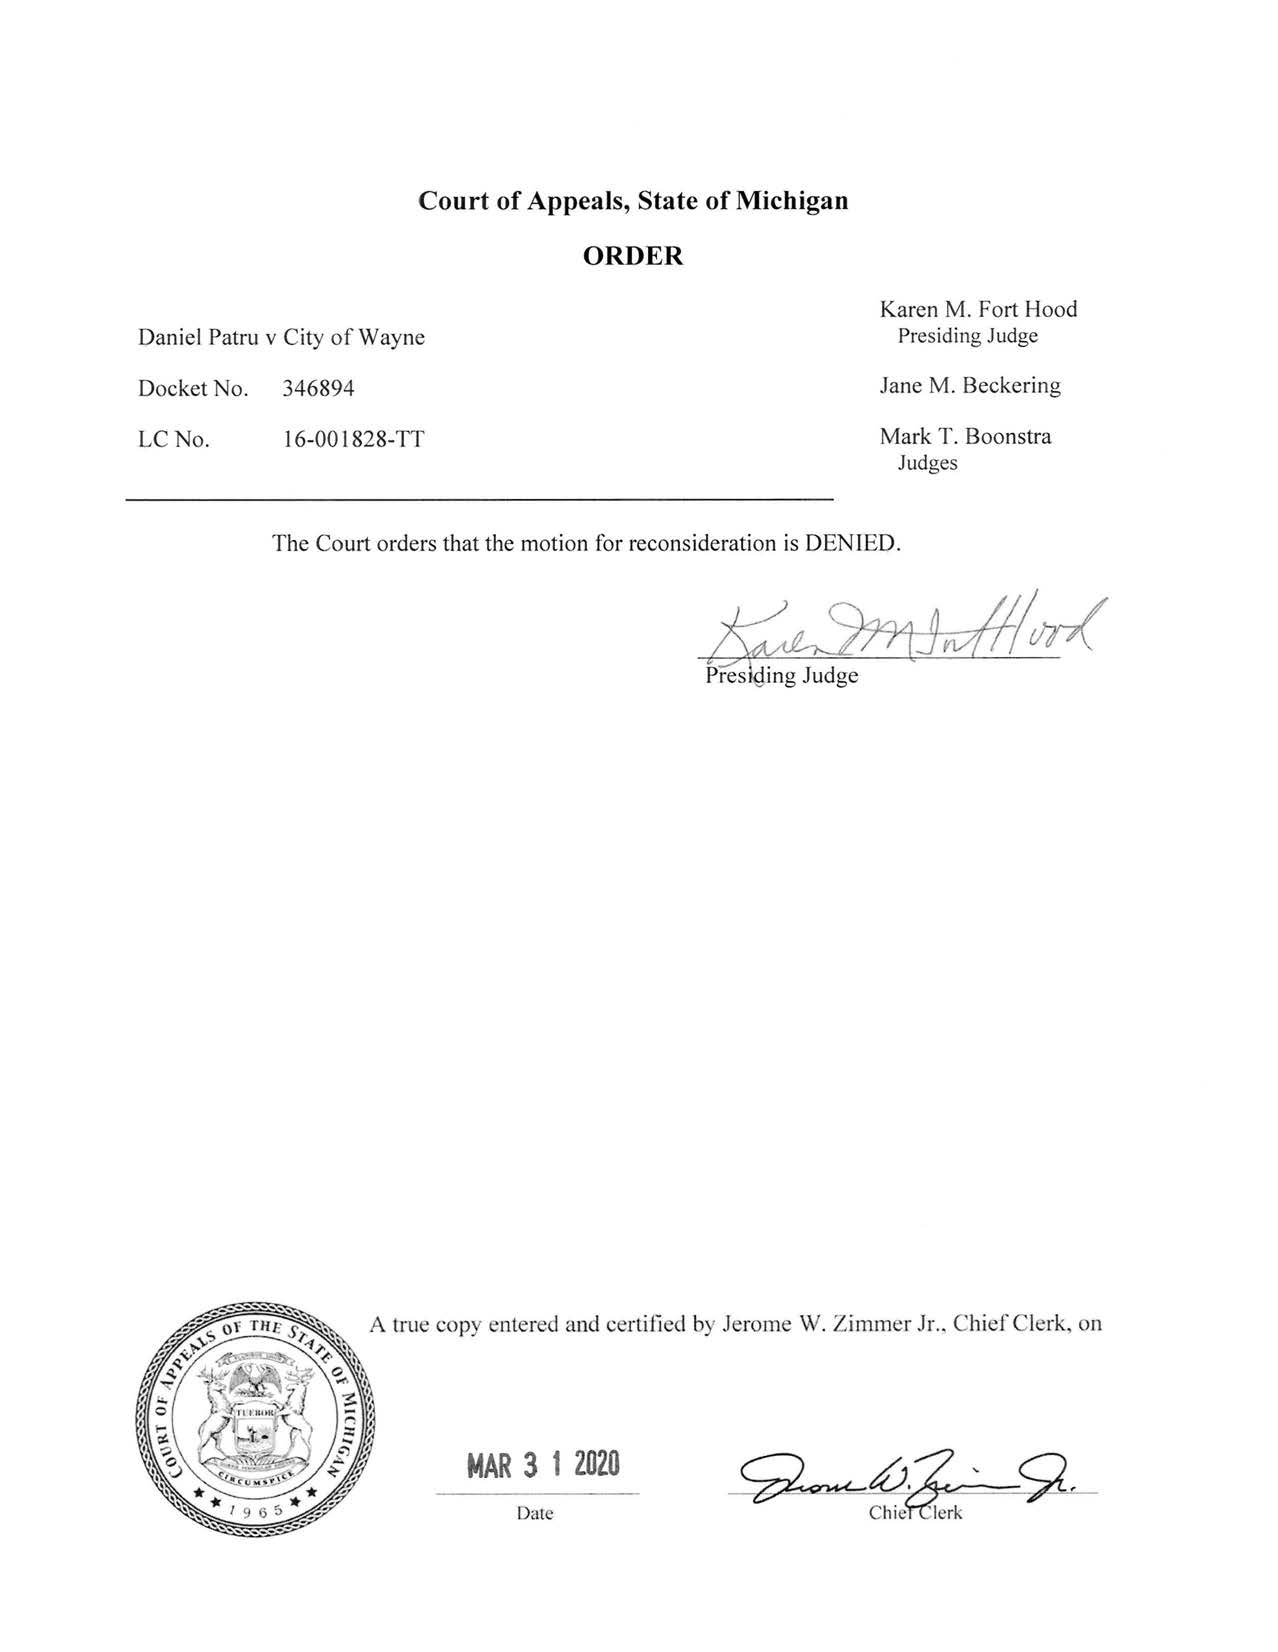
\includepdf[frame,scale=0.7,pagecommand={},pages=-]{appendix/patru2-reconsiderationDenied.pdf}
% \section{Copy of Court of Appeals' 2nd Opinion (2020)}
% 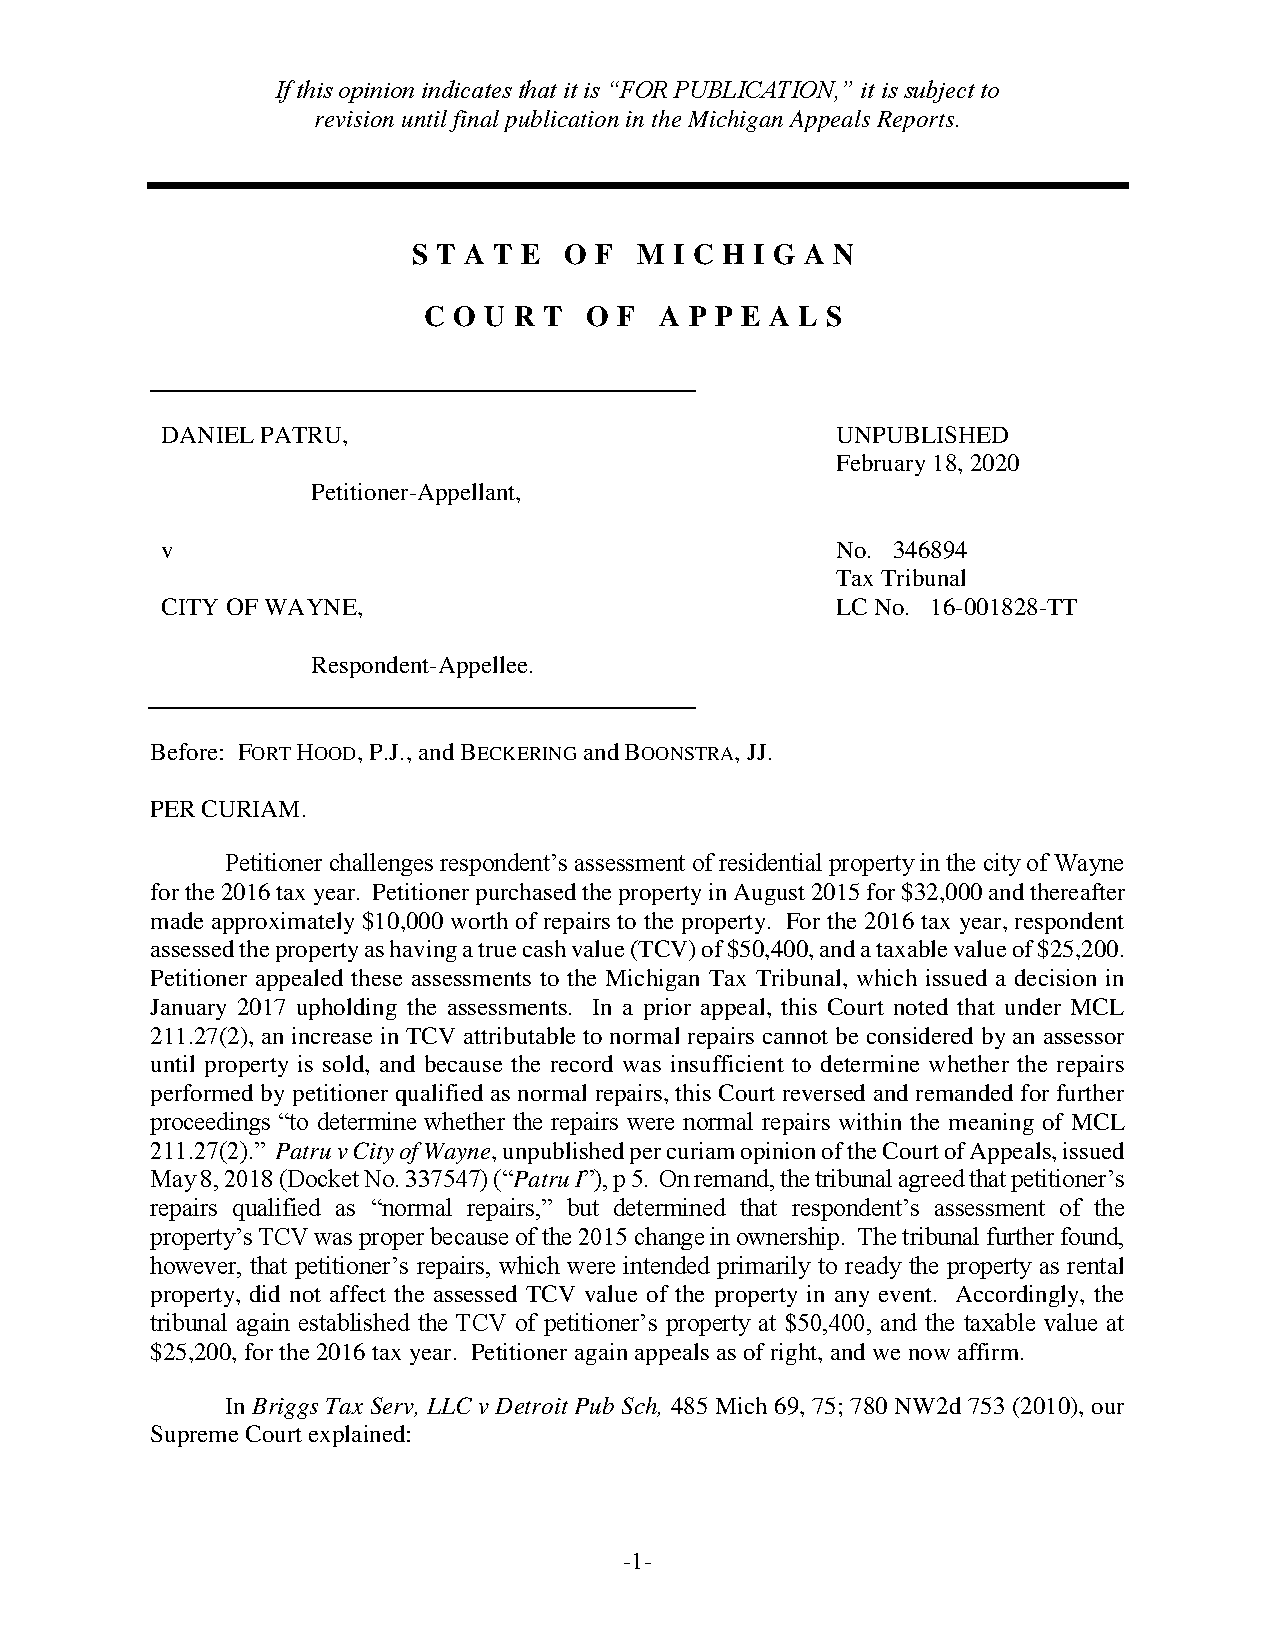
\includepdf[pages=-]{appendix/patru2.pdf}
% \section{Copy of Court of Appeals' 1st Decision (2018)}
% 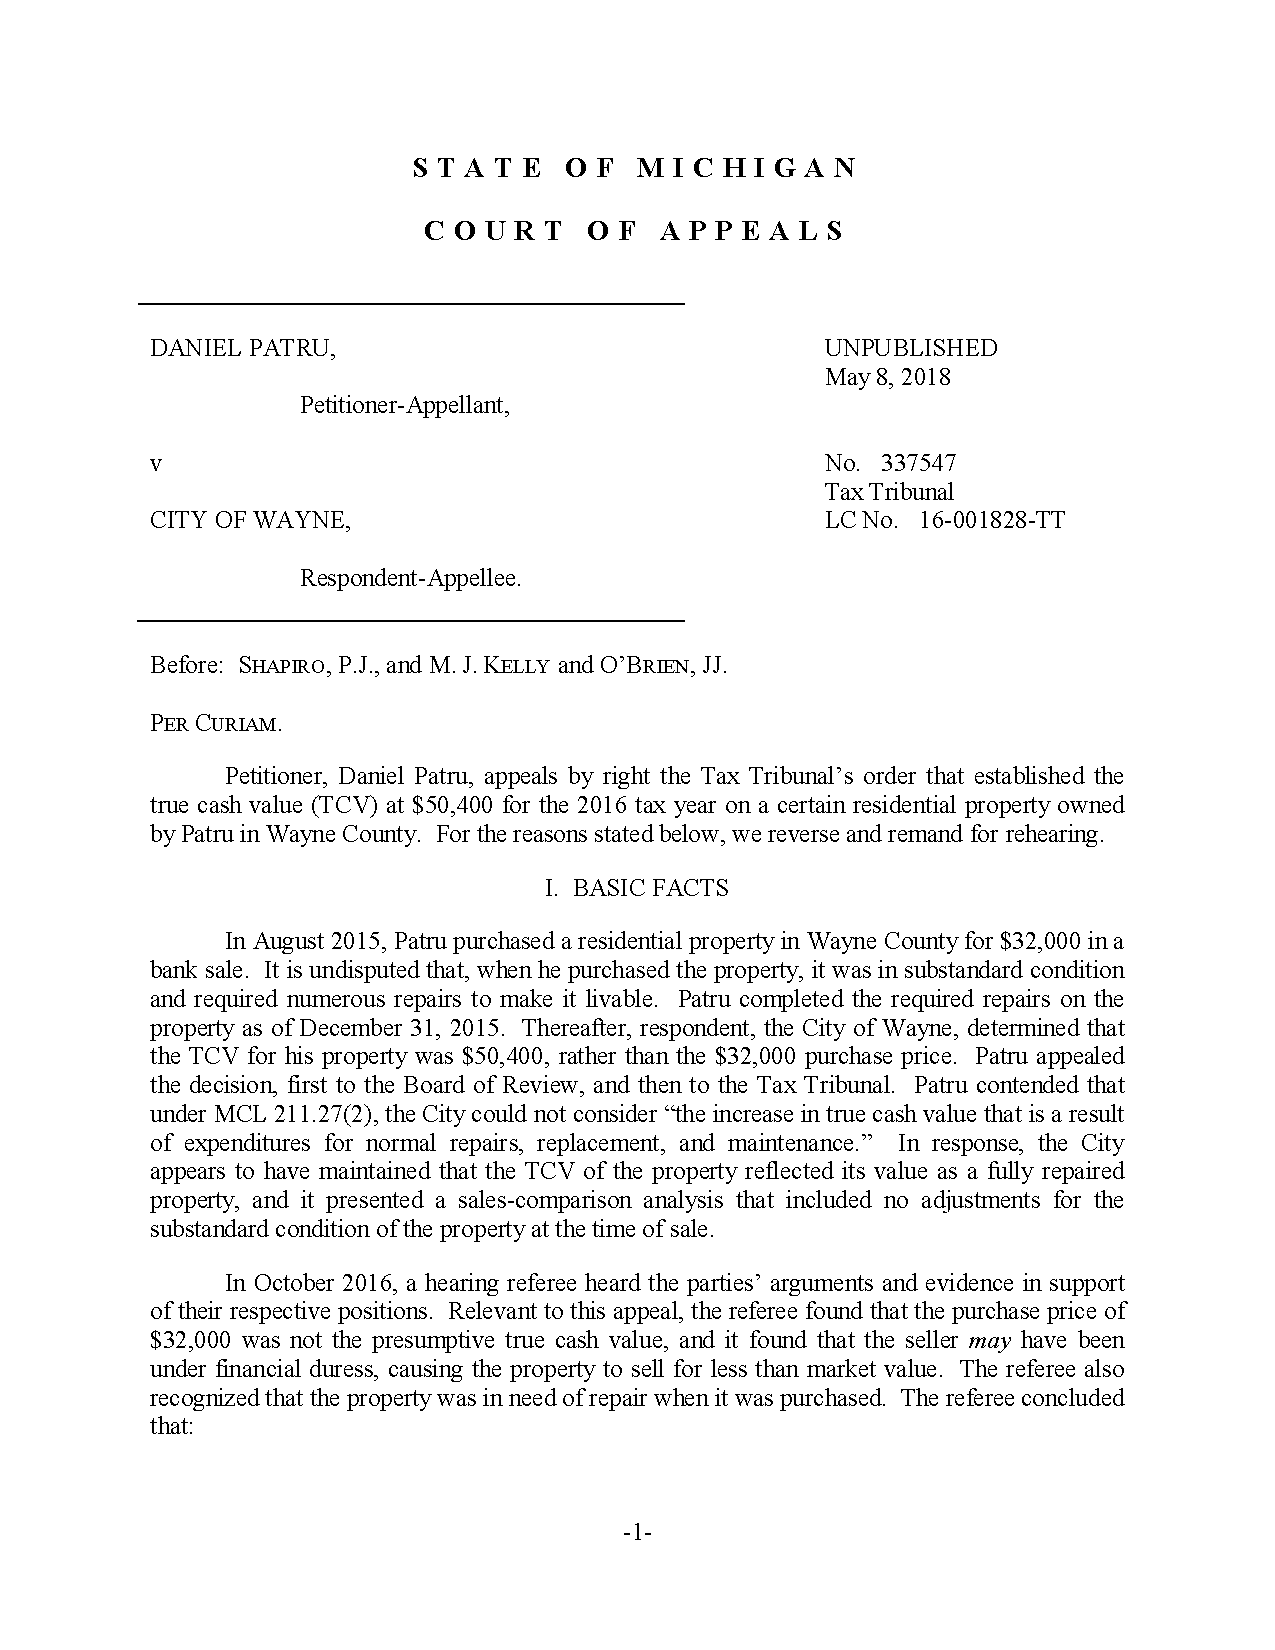
\includepdf[pages=-]{appendix/patru1.pdf}

%%% Local Variables:
%%% mode: latex
%%% TeX-master: t
%%% TeX-command-default: Latex Make
%%% End:
\end{document}
